%
% File hicss.tex
%
% Contact: Holm Smidt, hicss@hawaii.edu
%%
%%
%% Based on the style files for ACL 2015 by 
%% car@ir.hit.edu.cn, gdzhou@suda.edu.cn


\documentclass[10pt]{article}


\usepackage[letterpaper]{geometry}
\usepackage{hicss}
\usepackage{times}
\usepackage[none]{hyphenat}
\usepackage{url}
\usepackage{latexsym}
\usepackage{minted}
\usepackage{indentfirst}
\usepackage{graphicx}
\graphicspath{{images/}}
\usepackage{filecontents}
\usepackage{hyperref}
\usepackage{amsmath}
\usepackage{filecontents}

\usepackage{hyperref}
\usepackage{amsmath}
\DeclareMathOperator*{\argmax}{argmax}
\DeclareMathOperator*{\argmin}{argmin}
\newcommand{\sansserifformat}[1]{\fontfamily{cmss}{ #1}}%

\setlength\titlebox{5cm}

% You can expand the titlebox if you need extra space
% to show all the authors. Please do not make the titlebox
% smaller than 5cm (the original size).


\title{Sentiment Analysis for Amazon Musical Instruments Reviews}

% Comment this for initial manuscript 
% Uncomment this for final manuscript
\author{Eduard Mihranyan \\
   {\underline{ mihranyaneduard@gmail.com}} \\}
%  Second Author \\
%  Affiliation \\
%  {\underline{ email@domain} }\\\And 
%  Third Author \\
%  Affiliation \\
%  {\underline{email@domain}} \\}

\date{}

\begin{document}
\maketitle
\begin{abstract}
{Sentiment analysis of product reviews, an application
problem, has recently become very popular in text mining
and computational linguistics research. Here, we want to
study the correlation between the Amazon product reviews
and the rating of the products given by the customers. We
use both traditional machine learning algorithms including Naive Bayes analysis, Support Vector Machines, XGBoost and deep neural networks such
as Recurrent Neural Network(RNN). By comparing these results, we could get a better understanding of the these algorithms. They could also
act as a supplement to other fraud scoring detection methods. 

\end{abstract}

\section{Introduction}

Recent years have seen an increasing amount of research
efforts expanded in understanding sentiment in textual resources. One of the subtopics
of this research is called sentiment analysis or opinion mining, which is, given a bunch of text, we can computationally study peoples opinions, appraisals, attitudes, and emotions toward entities, individuals, issues, events, topics and
their attributes. Applications of this technique are diverse.

For example, businesses always want to find public or consumer opinions and emotions about their products and services. Potential customers also want to know the opinions
and emotions of existing users before they use a service
or purchase a product. Last but not least, researchers\cite{Dave2003}
uses these information to do an in-depth analysis of market
trends and consumer opinions, which could potentially lead
to a better prediction of the stock market.

However, saying this, to find and monitor opinion sites
on the Web and distill the information contained in them
remains a formidable task because of the proliferation of
diverse sites. Each site typically contains a huge volume
of opinionated text that is not always easily deciphered in
long forum postings and blogs. The average human reader
will have difficulty identifying relevant sites and accurately
summarizing the information and opinions contained in
them\cite{Lui2012}. Besides, to instruct a computer to recognize sarcasm is indeed a complex and challenging task given that at
the moment, computer still cannot think like human beings.

The objective of this paper is to classify the positive
and negative reviews of the customers over different products and build a supervised learning model to polarize large
amounts of reviews. Our dataset consists of customers’ reviews and ratings, which we got from Amazon Musical Instruments Reviews. We extracted the features of our dataset
and built several supervised model based on that. These
models not only include traditional algorithms such as naive
bayes, linear supporting vector machines, XGBoost, but also deep learning metrics such as Recurrent Neural
Networks. We compared
the accuracy of these models and got a better understanding
of the polarized attitudes towards the products.
}


\section{Related Work}

So far, there are a lot of research papers related to product reviews, sentiment analysis or opinion mining. For example, Xu Yun \cite{Xu2015} et al from Stanford University applied
existing supervised learning algorithms such as perceptron
algorithm, naive bayes and supporting vector machine to
predict a review’s rating on Yelp’s rating dataset. They used
hold out cross validation using 70\% data as the training data
and 30\% data as the testing data. The author used different classifiers to determine the precision and recall values.
In paper\cite{Hota2018}, Maria Soledad Elli and Yi-Fan extracted sentiment from the reviews and analyze the result to build up a business model. They claimed that this tool gave them
pretty high accuracy. They mainly used Multinomial Naive
Bayesian(MNB) and support vector machine as the main
classifiers. Callen Rain\cite{Rain2013} proposed extending the current
work in the field of natural language processing. Naive
Bayesian and decision list classifiers were used to classify a
given review as positive or negative.

Deep-learning neural networks is also popular in the area
of sentiment analysis. Ronan Collobert\cite{Collobert2011} et al used a convolutional network for the semantic role labeling task with
the goal avoiding excessive task-specific feature engineering. On the other hand, in paper\cite{Socher2013}, the authors proposed
proposed using recursive neural networks to achieve a better understanding compositionality in tasks such as sentiment detection.

In this paper, we want to apply both traditional algorithms including Naive Bayesian,Support Vector Machine, XGBoost and deep-learning tricks. By comparing the accuracy of these models, we would like to get a better understanding how these algorithms work in tasks
such as sentiment analysis.

\section{Dataset and features}
\subsection{Data Preprocessing}

Our dataset comes from Amazon Musical Instruments Reviews\footnote{\url{https://www.kaggle.com/eswarchandt/amazon-music-reviews}}. This dataset has 10261 points in total.Each example includes the reviewer ID, name, helpfulness, review, summary time as well as the rating of the product. To better
utilize the data, first we extract the rating and review column since these two are the essential part of this project.
Then, we join review text with summary text. 

Besides, to have a brief overview of the dataset, we have
plot the distribution of the ratings. Figure 1 shows the distribution of ratings in our dataset. We can observe that the classes are highly imbalanced, i.e. class 1 and class 2 have small amount of data
while class 5 has more than 7000 reviews.

In the subsection ‘3.3 Features’, we will illustrate how
we convert a review text into an input vector. The target vector will be binary 1-good if the rating is higher than 3 and 0-bad if the rating is less than or equal to 3. 


\begin{figure}[thb]
	% Use the relevant command to insert your figure file.
	% For example, with the graphicx package use
    \centering
	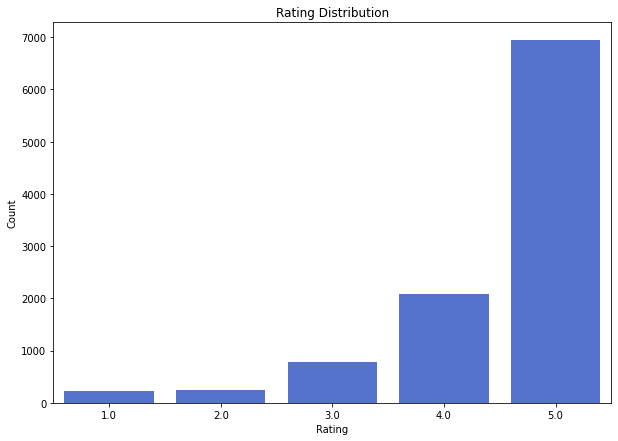
\includegraphics[clip,width=0.9\linewidth]{figure1}
	% figure caption is below the figure
	\caption{Rating Distribution of Amazon Review}
	\label{fig: sample-figure}       % Give a unique label
\end{figure}

  

\subsection{Data Resampling}

Due to the imbalance of our dataset, we have tried data
resampling in some of our experiments. Data resampling
is a popular way of dealing with imbalanced data. In this
project, we tried to oversample the minority class using SMOTE. However, since there are many
repeated samples in the training set, it is easy for the models to overfit. And the results of all models were better without oversampling. 

\subsection{Features}

As out main feature for each user is text review we need to deal with them using natural language processing techniques. We first removed punctuation, then we tokentized the sentences in the text, and eventually lemmatized each word to its lemma. We have used keras Tokenizer and converted texts to sequences. We have also done padding to equalize the lengths of all input reviews. As we were going to use LSTM too, it needs all inputs to be same length. Therefore reviews woth length less than max length will be made equal using extra zeros at end.

\section{Models}
\subsection{Naive Bayes}

Naive Bayes is one of the most common generative
learning algorithms for classification problems. This algorithm assumes that $x_i'$s are conditionally independent given y, which is called Naive Bayes assumption.

\[p(x_1,...,x_k|y)=\prod_{i=1}^{k} p(x_i|y)\]

We also incorporated Laplace Smoothing in our model to
make it work better. The prediction of an example is given
by the formula below:

\[\hat{y}^{(i)}=\argmax_j\prod_{i=1}^{k} p(x_i|y=j)\phi(j)\]

With the first way of representing review texts, it takes an
array of non-negative integers, and models $p(x_i|y)$ with
multinomial distribution. With the second way of representing review texts using glove dictionary, the inputs are no longer non-negative integers, so we chose to model $p(x_i|y)$
with Gaussian distribution.

\subsection{Logistic Regression}
Logistic regression, a common binary classification algorithm, utilizes the sigmoid function (also known as the logistic function). Incorporated with linear prediction parameters, $\theta$ and the features of $x$, the classification prediction
is given by the following probability distribution:

\[h_{\theta}(x)=\frac{1}{1+e^{-{\theta}^{T}x}}\]

whose log likelihood is given by the following:

\[l(\theta)= \sum_{i=1}^{m}y^{(i)}\log h(x^{(i)})+(1-y^{(i)})\log (1-h(x^{(i)}))\]

\subsection{Linear Support Vector Machine}

Linear SVM is a mthod that creates a classifier(a vector)
that separates the labeled datasets. Geometrically given two
types of points, circles and x’s, in a space, it tries to maximize the minimum distance from one of the points to the other. In other words, it maximizes the margin. The optimization problem that SVM tried to solve is below:


\[\argmax_{\gamma,\omega,b}\frac{1}{2}\left\|\omega\right\|^2\]
\[s.t. y^{i}(w^{T}x+b)>=1,i=1,2,...,m\]

It tried to find the w to satisfy the maximum margin problem and satisfy the separability constraint.

\subsection{XGBoost classifier}

XGBoosting is another popular ensemble
method used for regression and classification. Given a training
sample ($x, y$), the goal is to find a function $F^{*}(x)$ that maps $x$ to
$y$ such that the expected value of some loss function $\Psi(y, F(x))$
is minimized. Boosting approximates $F^{*}(x)$ by the following
equation:

\[F(x) = \sum_{m=1}^{M}\beta_mh(x;a_m)\]

where the functions $h(x; a_m)$ (called “base learners”) are simple
functions of $x$ with parameters $a$. Starting with $F_0(x)$, the
parameters $\beta_m$ and $a_m$ are found in a “stage-wise” manner and
the function $F_m(x)$ is updated as:

\[F_m(x) = F_{m-1}(x)+\beta_mh(x;a_m)\]

In tree boosting, the base learner $h(x; a)$ is an $L$-terminal node
regression tree. At each iteration $m$, a regression tree partitions
the $x$-space into $L$-disjoint regions $\{R_{lm}\}_{l=1}^{L}$ and predicts a
separate constant value in each one. The update rules for
calculating $F_m(x)$ given $F_{m−1}(x)$ are as follows:

\[\tilde{y}_{im}=\left[ \frac{d\Psi(y_i,F(x_i))}{d F(x_i)}\right]_{F(x)=F_{m-1}(x)}\]
\[\bar{y}_{lm}= mean_{x_i\in R_{lm}}(\tilde{y}_{im})\]
\[h(x;\{R_{lm}\}_1^L)=\sum_{l=1}^{L}\bar{y}_{lm}1(x\in R_{lm})\]
\[\gamma_{lm}= \argmin_{\gamma}\sum_{x_i\in R_{lm}}{\Psi(y_i,F_{m-1}(x_i)+\gamma)\]
\[F_m(x)=F_{m-1}(x)+\nu\gamma_{lm}1(x\in R_{lm})\]

\subsection{Long Short Term Memory}

Long Short Term Memory(LSTM) is unit of Recurrent Neural Network(RNN). A common LSTM unit is composed of a cell, an input gate, an output gate and a forget gate. The cell remembers values over arbitrary time intervals and the three gates regulate the flow of information into and out of the cell. LSTM networks are well-suited to classifying, processing and making predictions based on time
series data, since there can be lags of unknown duration between important events in a time series. The configuration is shown as the Figure 2 below.

\begin{figure}[thb]
	% Use the relevant command to insert your figure file.
	% For example, with the graphicx package use
    \centering
	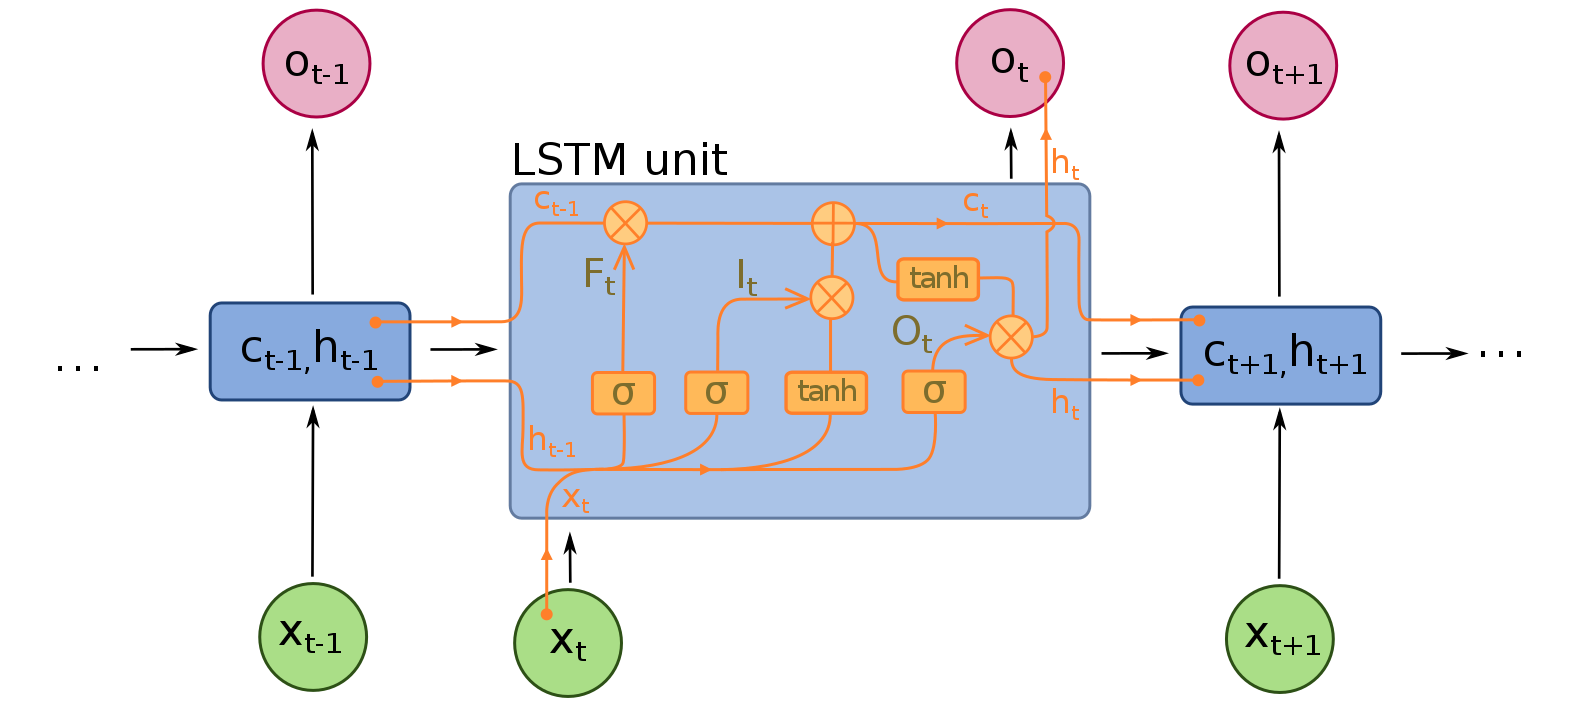
\includegraphics[clip,width=0.9\linewidth]{figure2}
	% figure caption is below the figure
	\caption{Long Short Term Memory}
	\label{fig: sample-figure}       % Give a unique label
\end{figure}

We have used the following network architecture: a Embedding layer, two LSTM layer, one Dense layer of ReLU, a Dropout layer and final sigmoid layer for binary classification. This architecture is specially designed to work on sequence data. It fits perfectly for many NLP tasks like tagging and text classification. It treats the text as a sequence rather than a bag of words or as ngrams.


\section{Results and Discussion}
\subsection{Results}

The entire dataset of 10,261 reviews was divided into a training set of size 8208 (80\%)and a test set of size 2053 (20\%).

With 2067-d input features representing review text, we implemented Multinomial Naive Bayes, SVM with Linear Kernel, Logistic Regression, XGBoost and LSTM. As our data set is highly imbalanced the accuracy score will not be the best metric choice. So we will also consider a roc\_auc score and f1 scores for both classes. We have used weight balancing in Logistic Regression and XGBoost to penalize mistakes on minority class. 

Multinomial Naive Bayes perform better than Logistic Regression and SVM in all metrics. XGBoost has an advantage towards predicting the majority class, however it poorly predicts the minority class in terms of f1 score. LSTM performs best of all of them in every metric.  


\begin{center}
\begin{tabular}{ l|c|c|c} 
  Models & Accuracy & F1 score & ROC  \\
 \hline
 Multinomial NB & 80.4\% & 0.52 & 0.52  \\ 
 Logistic Regression & 51.7\% & 0.43 & 0.51  \\ 
 Linear SVM & 79.0\% & 0.52 & 0.52 \\ 
 XGBoost & 88.4\% & 0.50 & 0.52 \\ 
 XGBoost+SMOTE & 82.0\% & 0.53 & 0.53 \\ 
 LSTM & 86.8\% & 0.69 & 0.72 \\
 LSTM+SMOTE & 87.3\% & 0.72 & 0.74 \\
 \hline

\end{tabular}
\bigskip
Table1. Performance of different models
\end{center}

The XGBoost classifier seems to be overfitted as it has high accuracy and low F1 score. Given that the data has almost 90\% of negative class it doesn't learn to properly predict the minority class. The Logistic Regression was underfitted due to balancing the data with class weighting. As we can see from the table of performance LSTM with SMOTE gives significantly higher F1 score and ROC. 

\subsection{Discussion}
We have tried also other standard methods of processing text data such as count vectorizing and tf-idf vectorization. However it doesn't gave good results. We also tried to add as a feature the length of a review text and it doesn't improve our metrics of evaluation. The hyper-parameter tuning was also used for XGBoost and SVM which did not help these models to perform better. 

Another technique that was used improve results of classification was SMOTE. It synthetically generates new data points of minority class assuming that points in one class are nearly located in terms of euclidean distance. However, almost all models' results shrunk down. It can be because new data points were not so informative and algorithms were overfitted on the training set.     



\section{Conclusion and Future Work}

In summary, we have tried two types of features. For this two type of features, we tried all the algorithms we mentioned in the model part including Naive Bayes, SVM,
Logistic Regression, XGBoost, LSTM. From the results, we can see that our accuracy, F1 score and ROC score on the test set is the best when we use LSTM. One of the main reason our accuracy is not high enough is because of the data imbalance. We tried resampling and different weighting techniques. But that didn’t help too much. Another possible solution we haven’t tried is to find more data points from other resources. We think that might help us solve the problem of data imbalance.
 

%Bibliography 
\bibliographystyle{ieeetr}

\begin{thebibliography}{9}
{
\bibitem{Dave2003} 
K. Dave, S. Lawrence, and D. M. Pennock. Mining the
peanut gallery: Opinion extraction and semantic classification
of product reviews. In \textit{Proceedings of the 12th international
conference on World Wide Web}, pages 519–528. ACM, 2003..

\bibitem{Lui2012} 
B. Liu and L. Zhang.\textit{A Survey of Opinion Mining and Sentiment Analysis}, pages 415–463. Springer US, Boston, MA,
2012.

\bibitem{Xu2015} 
Y. Xu, X. Wu, and Q. Wang. Sentiment analysis of yelps
ratings based on text reviews, 2015.

\bibitem{Hota2018} 
S. Hota and S. Pathak. Knn classifier based approach for
multi-class sentiment analysis of twitter data. In \textit{International
Journal of Engineering Technology}, pages 1372–1375. SPC,
2018.

\bibitem{Rain2013} 
C. Rain. Sentiment analysis in amazon reviews using probabilistic machine learning. \textit{Swarthmore College}, 2013.

\bibitem{Collobert2011} 
R. Collobert, J. Weston, L. Bottou, M. Karlen,
K. Kavukcuoglu, and P. Kuksa. Natural language processing (almost) from scratch. \textit{Journal of Machine Learning
Research}, 12(Aug):2493–2537, 2011.}

\bibitem{Socher2013} 
R. Socher, A. Perelygin, J. Wu, J. Chuang, C. D. Manning,
A. Ng, and C. Potts. Recursive deep models for semantic
compositionality over a sentiment treebank. In \textit{Proceedings
of the 2013 conference on empirical methods in natural language processing}, pages 1631–1642, 2013.

\end{thebibliography}
\end{document}
